\documentclass[11pt, a4paper]{article}

\usepackage[utf8]{inputenc}
\usepackage[T1]{fontenc}
\usepackage[a4paper, margin=2.5cm]{geometry}
\usepackage[spanish, es-nodecimaldot]{babel}

% Fuente Sans-Serif nativa garantizada en TeX Live
\usepackage{lmodern}
\renewcommand{\familydefault}{\sfdefault}

\usepackage{enumitem}
\setlist[itemize]{label=-}

\usepackage{graphicx}
\usepackage{microtype}
\usepackage[hidelinks]{hyperref}

\hypersetup{
    colorlinks=true,
    linkcolor=black,
    citecolor=black,
    urlcolor=blue
}

\setlength{\parindent}{1.2em}
\setlength{\parskip}{0.45em}

\title{\textbf{Reporte de Modelado e Implementación\\Sistema de Chat Concurrente}}
\author{Facultad de Ciencias, UNAM}
\date{\today}

\begin{document}

\maketitle

\begin{abstract}
Se presentan las decisiones de modelación e implementación tomadas para concretar un programa de Chat con un Servidor y múltiples clientes implementados en Go y Vala respectivamente. Los programas se comunican mediante Sockets y usando como protocolo de mensajes a Json.
\end{abstract}

\section*{Introducción}

Dadas un conjunto de especificaciones establecidas en el protocolo del proyecto, se implementó un chat en el que múltiples clientes pueden conectarse concurrentemente e interactuar entre sí por intermedio del servidor. En particular, la ejecución del programa se da de forma concurrente mediante hilos de ejecución y con JSON como el protocolo de comunicación entre los elementos del programa.

La implementación del Servidor, y el conjunto de structs auxiliares a él, se hizo en el lenguaje programación Go, mientras que el Cliente fue implementado en Vala. De esta forma, para conseguir la implementación del primero se crearon un total de 8 structs, en tanto que para el segundo un total de 10 clases.

La estrategia para conseguir la implementación se fundamentó en conseguir un Servidor funcional primeramente, dada la mayor cantidad de responsabilidad asociadas a él y el desconocimiento general del lenguaje en que se implementó, para, una vez conseguido un Servidor funcional, implementar el Cliente, dadas la menor cantidad de responsabilidades a él y el relativo parecido que tiene Vala respecto de Java.

En la siguiente sección se describe el proceso de modelado del programado junto con las decisiones de implementación más importantes.

\section*{Desarrollo}

En esta sección se describe la modelación del Cliente y del Servidor, para posteriormente indicar cómo dicho modelo se implementó en los respectivos lenguajes.

En el trabajo para conseguir la implementación solicitada, se tomó la decisión de enfocar los esfuerzos iniciales en diseñar el servidor. Dicha elección se sustentó en el papel de coordinación que tiene, pues sirve de punto de conexión para todos los usuarios; garantiza la consistencia entre el estado del chat; y asegura que se cumpla el protocolo de comunicación y de conexión. En este sentido, el modelado de Cliente estuvo sujeto a las decisiones de diseño tomadas para el Servidor.

\subsection*{Modelado}

\subsubsection*{Servidor}

La construcción del modelo para el Servidor se dio en dos fases. En la primera se identificaron los objetos que deberían conformar al proyecto, así como las responsabilidades asociadas a cada uno, basándose tanto en las especificaciones de implementación del protocolo como en la explicación de implementación expuestas por Becerril Fuentes~\cite{becerril2019}, mientras que en la segunda se refinó dicha identificación al analizar la implementación propuesta en el libro de Viso y Peláez~\cite{viso2012}, con lo cual se consiguió un diseño más robusto al poder definir de forma más clara y completa el comportamiento asociado a cada objeto.

De la especificación mostrada en las notas de Becerril Fuentes~\cite{becerril2019} se identificaron directamente los objetos Conexión y Mensaje; el primero encargado de enviar mensajes al Cliente y de recibirlos de él, mientras que el segundo de tener la estructura especificada en el protocolo del proyecto para los mensajes. Al considerar la idea de un objeto Mensaje, se derivó directamente la idea de tener dos objetos relacionados al Mensaje: 1) un Builder de Mensaje encargado de construir los distintos tipos de mensajes que el Servidor puede enviar a los clientes como respuesta a sus solicitudes y a los sucesos producidos por las acciones del resto de usuarios y 2) un Parser de Mensaje encargado de identificar el tipo de Mensaje enviado por el Cliente y, una vez identificado, descomponerlo en los campos que, de acuerdo al protocolo, cada uno de ellos debe tener, con lo cual conseguir atender sus peticiones de forma adecuada.

Adicionalmente, se atendió la sugerencia del libro de modelado y se crearon los objetos Sala y Usuario, ambos auxiliares a Servidor. El primero literalmente una sala de la cual diversos usuarios son parte, y la segunda para almacenar la información asociada a cada Cliente que establece Conexión con el Servidor.

Sobre el comportamiento, primero se prestó atención al más general e intuitivo que debería de tener el Servidor:
\begin{itemize}
    \item Debe inicializarse, en el sentido de que tiene que empezar a esperar conexiones de los clientes y gestionar dichas conexiones.
    \item Debe enviar mensajes a los clientes y recibirlos de ellos.
    \item Tiene que procesar y cumplir las peticiones que los clientes envían por medio de los mensajes.
\end{itemize}

De esta primera fase detectaron comportamientos adicionales auxiliares a los principales. En particular:
\begin{itemize}
    \item Verificar que los usuarios que buscan conectarse no estén conectados desde antes
    \item Desconectar a usuarios
\end{itemize}

Dado que el envío y recepción de mensajes es el comportamiento propio de Conexión, se decidió que las funciones de Servidor encargadas de eso usaran instancias de Conexión para poder cumplir con el envío de mensajes del Servidor al Cliente y de la recepción de mensajes del Cliente. Así, a la clase Conexión le fueron asociados los comportamientos:
\begin{itemize}
    \item Envío de Mensajes al Cliente, los cuales se envían como bytes para poder usar a los sockets y que su contraparte sea capaz de entender lo que recibe. Para esto, recibe un mensaje que está a un paso de construirse, el cual es transformado a bytes respetando el protocolo Json.
    \item Recepción de Mensajes que envía el Cliente, los cuales se reciben como bytes y se devuelven así.
\end{itemize}

Los mensajes con los que trabaja la Conexión son potencialmente distintos, en el sentido de que cada tipo de mensaje tiene campos distintos. Por esta razón se decidió crear la interfaz Mensaje, la cual declara una función que devuelve el tipo de mensaje. A partir de ella, se decidió crear un struct por cada tipo de mensaje especificado en el protocolo, en donde cada uno de ellos implementa la función prometida por la interfaz devolviendo su tipo. Con esto especificado, se formaron los structs mensaje A Cliente Builder y mensaje De ClienteParser.

El comportamiento en mensaje A Cliente Builder está encaminado construir parcial mensajes o agregarles campos con sus respectivos valores, así como generar el JSON final, un vez agregada toda la información para identificar un mensaje y para especificar sus campos.

En mensaje DeClienteParser se procesa el flujo de bytes recibido por la Conexión y se lee como un mensaje. Se usa dicho mensaje para identificar su tipo y devolver el tipo específico de mensaje.

\begin{figure}[htbp]
    \centering
    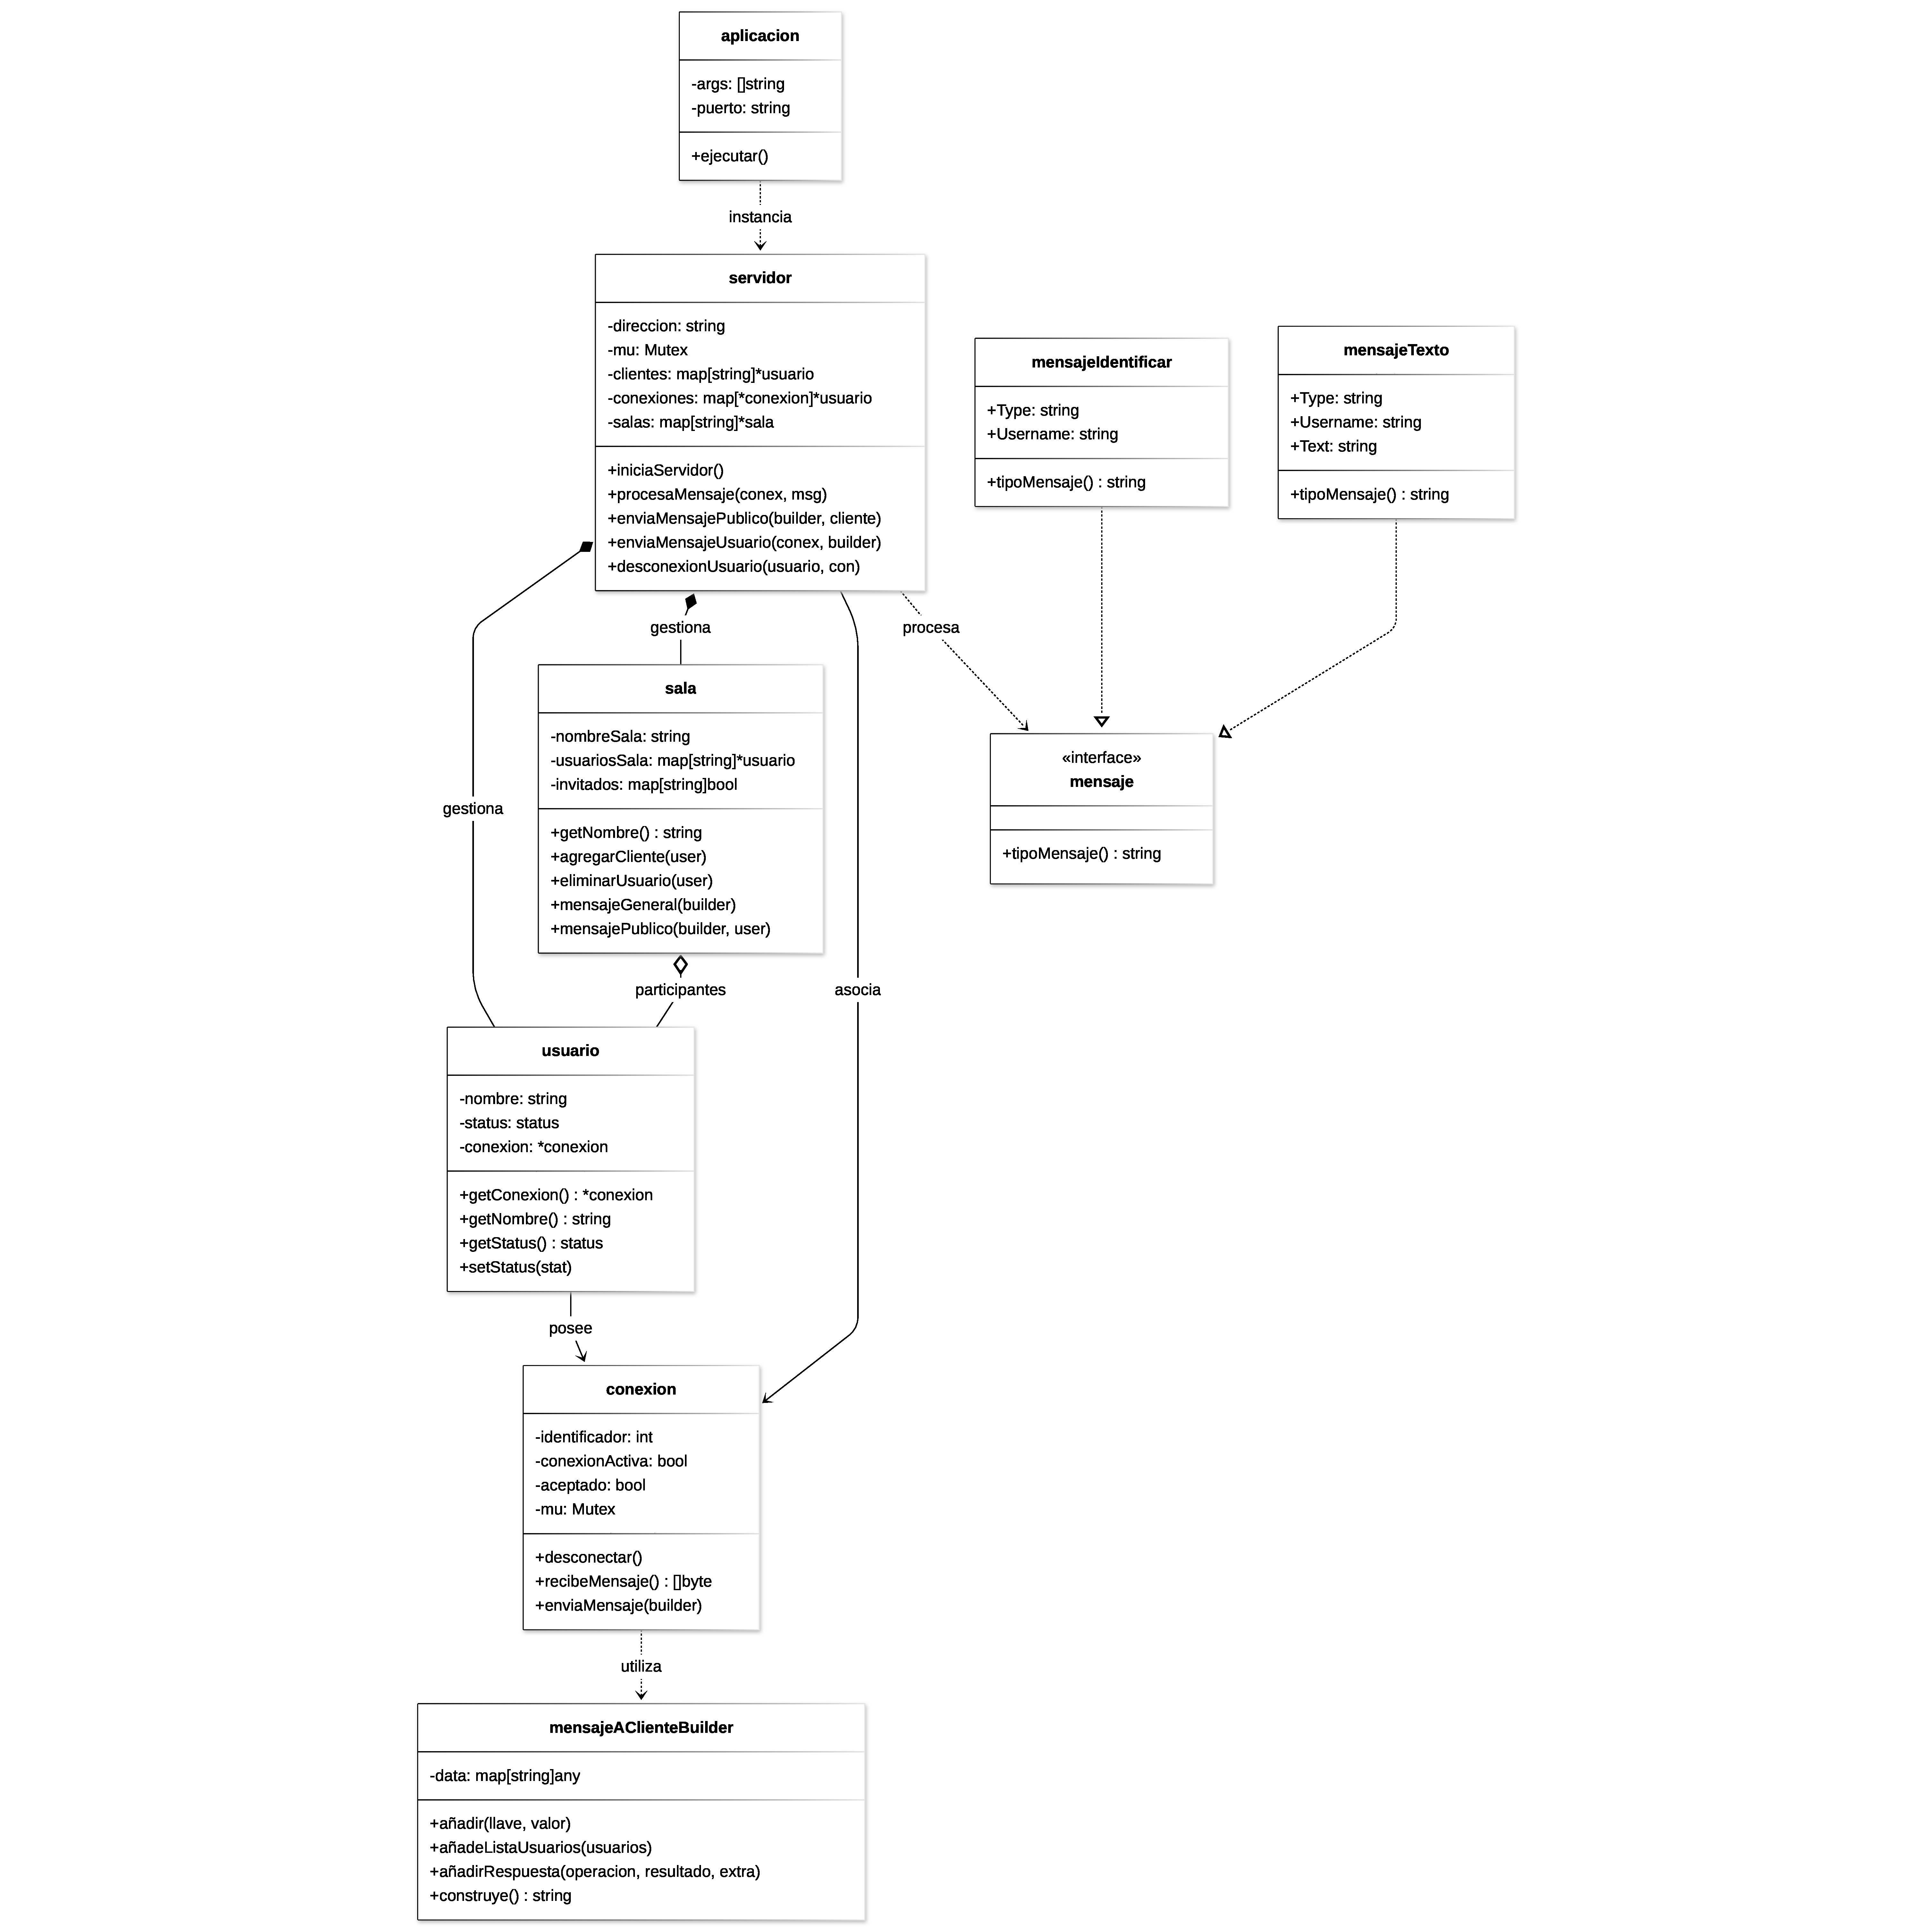
\includegraphics[width=0.85\textwidth]{../diagramas/diagramaDeClasesServidor.pdf}
    \caption{Diagrama de clases y relaciones de los componentes del Servidor en Go.}
    \label{fig:diagrama_servidor}
\end{figure}

\subsubsection*{Cliente}

Las ideas para modelar el Cliente se derivaron del modelo del Servidor. Nuevamente se consultaron las especificaciones en los textos de Peláez~\cite{viso2012} para refinar la asignación de responsabilidades entre los objetos y el comportamiento de cada uno.

Así, al Cliente se le asoció el comportamiento:
\begin{itemize}
    \item Inicializar el Cliente para recibir mensajes del Servidor, como respuesta a las propias peticiones del cliente y a los sucesos generados por el resto de clientes conectados, y para recibir en la terminal los mensajes que el usuario del programa Cliente quiere enviar.
    \item Procesar los mensajes del servidor para poder hacerle saber al usuario del programa las respuestas que recibe a sus peticiones y de los sucesos generados por el resto de clientes conectados.
    \item Enviar mensajes por intermedio de la Conexión.
    \item Desconectar al cliente, para que deje de recibir mensajes del Servidor
\end{itemize}

El procesamiento de mensajes se vale nuevamente de un parseados de mensajes: Mensaje DeServidorParser, cuyo comportamiento es análogo al parseador presente en el servidor, con la diferencia que parsea únicamente mensajes de respuesta o de sucesos. Para esto, nuevamente se hizo uso de la interfaz Mensaje, la cual sirve para poder acceder a las propiedades asociadas a cada tipo de mensaje (propiedades en términos de los campos que la componen), con lo cual al procesar mensajes, Mensaje De Servidor Parser devuelve el tipo Mensaje.

El envío y recepción de mensajes hacia y del Servidor nuevamente se especifican en un objeto Conexión. Así, el comportamiento asociado a este objeto es:
\begin{itemize}
    \item Recibir mensajes enviados como JSON por el servidor mediante el enchufe como un flujo de bytes y lo devuelve como un string.
    \item Enviar mensajes al servidor con el formato JSON como un flujo de bytes.
\end{itemize}

A diferencia de las responsabilidades asociadas al Servidor, el cliente debe poder recibir constantemente mensajes que el usuario del programa quiera enviar al Servidor, así como mostrarle a él directamente los mensajes de respuesta del Servidor. Este comportamiento en un primer momento pareció idéntico al realizado por Conexión, sin embargo, se concluyó que, pese a parecerse en términos de la necesidad de construir y parsear mensajes, estos provenían de una fuente distinta y su gestión no era idéntica, tal y como sí sucede con Mensaje De ServidorParser.

En consecuencia, se tomó la decisión de crear una la clase Consola, encargada de gestionar la comunicación con la terminal. Así, se le dio el comportamiento:
\begin{itemize}
    \item Leer las banderas y campos desde la terminal que constituyen los posibles mensajes que el Cliente puede enviar al Servidor y, de ser correctos, despachar a parsearlos para que se puedan ejecutar correctamente las peticiones contenidas en los mensajes.
    \item Mostrar en la terminal los mensajes que se reciben del Servidor, para que el Cliente pueda estar enterado.
\end{itemize}

La estrategia de construcción de mensajes y de su parseo desde la consola es análoga a la seguida en el Servidor y en Mensaje De ServidorParser, con la diferencia de que la intención al parsearlo es mostrarle en la terminal al usuario del programa los mensajes de notificación enviados por el Servidor y recibir directamente de ella la información sobre el tipo de mensaje, y los campos asociados a él, que el usuario quiere enviar. Evidentemente, ambos comportamientos están estrechamente vinculados.

Se determinó que, cada vez que fueran recibidos mensajes, la clase ConsolaParser tomará las cadenas de texto y verificara que fuera un mensaje válido, en términos la bandera contenida en el mensaje y la información asociada a dicha bandera, hecho siguiendo la misma estrategia que en los parseadores de mensaje de Cliente y Servidor. Para cada posible bandera, en la clase ConsolaBuilder se definió un método que construye el JSON asociado a ella. En este sentido, ConsolaBuilder facilita la construcción de mensajes, sirviendo de intermediario entre ConsolaParser y la clase MensajeAServidor Builder, siendo este último el verdadero encargado de construir los mensajes respetando el protocolo JSON. Esta última clase es análoga a MensajeAClienteBuilder de Servidor.

\begin{figure}[htbp]
    \centering
    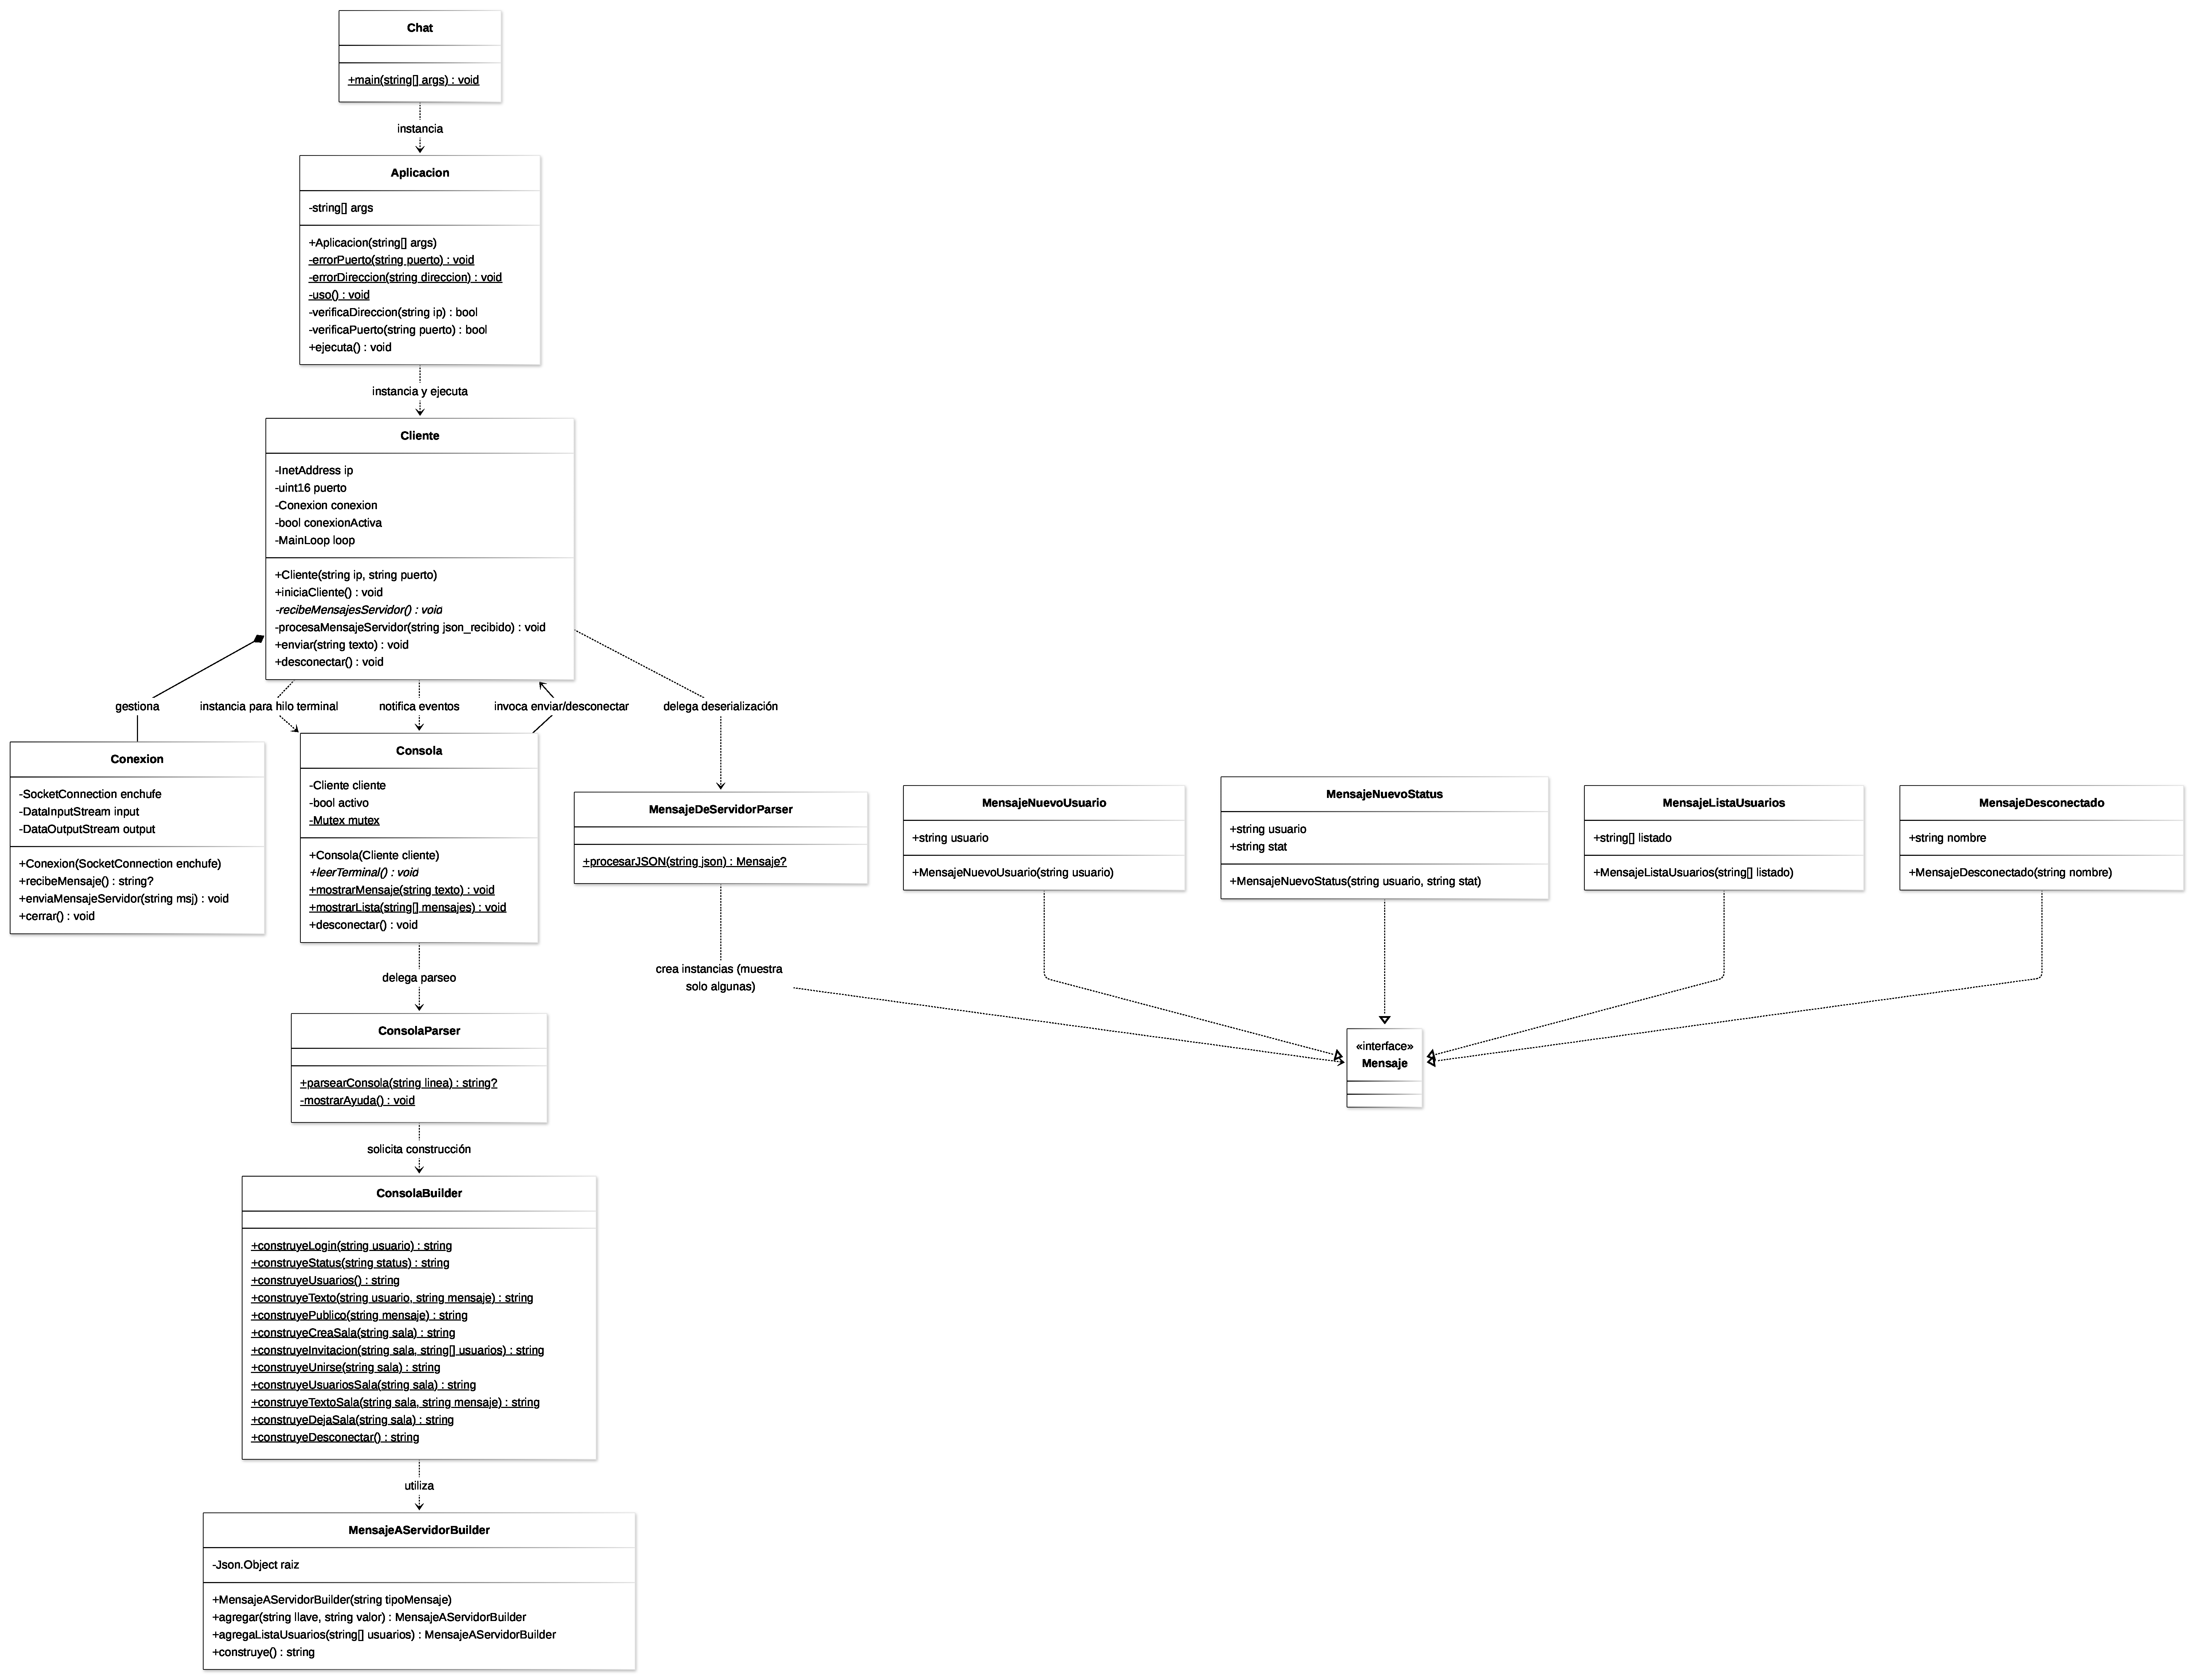
\includegraphics[width=0.85\textwidth]{../diagramas/diagramaDeClasesCliente.pdf}
    \caption{Diagrama de clases y relaciones de los componentes del Cliente en Vala.}
    \label{fig:diagrama_cliente}
\end{figure}

\subsection*{Implementación}

Para decidir los lenguajes de programación a utilizar se tomó en cuenta la intención de aprender nuevos lenguajes al mismo tiempo de reconocer la posibilidad de que una elección incorrecta con toda seguridad haría incrementar la dificultad del proyecto. Por lo tanto, la elección quedó sujeta a las facilidades que ofreciera la documentación y la comunidad alrededor de los lenguajes en lo que respecta a la implementación de Sockets para clientes y usuarios y al uso de JSON.

La decisión se dio en un sentido contrario al modelado. Primero se tuvo certeza en qué usar para implementar el Cliente, y después se tuvo para el Servidor.

La elección de Go como lenguaje para el Servidor se debió a 1) Buenas referencias de personas que han implementado chats; 2) La presencia de concurrencia nativa mediante las Goroutines; 3) La disponibilidad de recursos en \textit{Go by Example}~\cite{gobyexample}, que, entre muchas otras cosas, muestra una implementación de las gorutinas y el uso de Json, lo cual facilitó enormemente la implementación. Adicionalmente, los recursos dispuestos en la especificación del lenguaje~\cite{gospec} fueron muy útiles.

Al respecto, es importante señalar que inicialmente se implementó una blockinqueue mediante los channels de Go para gestionar la ejecución de las peticiones de los clientes, para lo cual se había creado un struct tarea, que justamente representaba las tareas que tenían que ejecutarse. Sin embargo, esta decisión produjo problemas de inconsistencia, por lo cual se optó por usar Sync.Mutex para proteger los datos compartidos por las Conexiones y para la impresión de mensajes en la consola.

En tanto, para implementar los Mensajes, dado que en Go no cuenta con herencia de clases, se aprovechó el \textit{duck typing}~\cite{goducktyping}, donde múltiples eventos distintos de procesan bajo un contrato común. Así, cada tipo de mensaje del protocolo implementó la función tipo Mensaje(), permitiéndole devolver su tipo. Así, cualquier struct de mensaje pasó a ser automáticamente un mensaje válido, siendo aprovechado por la función procesa Mensaje() de Servidor.

Además, para poder acceder a los campos particulares de cada comando (por ejemplo, el campo username en mensajeldentificar) su uso el \textit{type switch}~\cite{gocomposite} el cual permite conocer el tipo dinámico de una variable asociada a una interfaz.

Sobre la construcción del Json, se usaron método que se encadenan para crearlos de forma dinámica, sin necesidad de tener una función que construya el Json asociado a cada tipo de mensaje.

Para el Cliente se optó por Vala dado que: 1) Se posee experiencia previa en Java, compartiendo entonces una sintaxis familiar, el enfoque a la programación orientada a objetos y la automatización de la gestión de la memoria; 2) El hecho de que el Cliente representa una menor cantidad de responsabilidades en relación al Servidor, lo cual dio pie a profundizar conocimientos en otro lenguajes para tareas desconocidas hasta el momento, lo cuál cumple con la intención de aprender un nuevo lenguaje; 3) La disponibilidad de documentación y de repositorios que dan información de calidad sobre el uso de Sockets y JSON, además de otros pormenores que resultaron muy útiles para conseguir una implementación exitosa.

Sobre este último punto, las fuentes más importantes para la fueron Valadoc~\cite{valadoc}, Wiki GNOME~\cite{gnomewiki} y el repositorio \textit{gtrophies} de Canek Peláez~\cite{gtrophies} para la construcción del Json.

La implementación de los Mensajes y del constructor/parseador de mensajes fue análoga a la hecha en Go.

\section*{Conclusiones}

El proyecto impuso diversos retos. Uno de los más significativos de todas residió en el modelado, pues se cayó en cuenta de que no solo se trata de abstraer objetos, propiedades y comportamientos, sino perfilar dicha abstracción hacia un esquema funcional que facilite la implementación. De esto, distintas decisiones iniciales sobre el modelo se descubrieron, con el avance de la implementación, insuficientes en el mejor de los casos. Por otro lado, los pormenores asociados a cada lenguaje fueron aspectos que no se consideraron inicialmente; la forma de compilar, organizar paquetes, estructurar código era algo que se tenía previsto, pero las especificidades fueron una gran sorpresa, sobre todo una vez que se ``tenían'' implementaciones terminadas y se intentaban probar; fue frustrante tener que posponer la prueba para resolver problemas de compilación inesperados. Además, usar las posibilidades dadas por cada lenguaje para darle forma al comportamiento de cada objeto fue muy retador; el Parser, Builder y los switch type fueron clases y comportamientos cuya construcción se hizo cuesta arriba. SI bien las bases fueron útiles, la necesidad de usar documentación e implementaciones previas fue la clave, sin esas fuentes habría resultado imposible conseguir programas funcionales.

El mayor aprendizaje obtenido fue: es bueno leer documentación y tratar de entender todos los pormenores del problema que se tiene enfrente, pero es mejor dedicar el doble del tiempo a implementar. El mayor problema que se tuvo fue dedicarle demasiado tiempo a leer, no porque sea malo, sino porque la implementación misma te hace descubrir huecos que al leer resultan imposibles de prever, ya sea porque literalmente no lees nada al respecto o porque, cuando lo lees, simplemente te parece irrelevante.

\begin{thebibliography}{99}

\bibitem{becerril2019}
Becerril Fuentes, Kimberly (2019). \textit{Notas para el curso de modelado y programación}. Facultad de Ciencias, UNAM. Recuperado de: \url{https://repositorio.unam.mx/contenidos/3640772}

\bibitem{viso2012}
Viso G., Elisa y Peláez V., Canek (2012). \textit{Introducción a las ciencias de la computación con Java} (2.ª~ed.). Facultad de Ciencias, UNAM. ISBN: 978-607-02-3345-6.

\bibitem{gobyexample}
\textit{Go by Example}. Recuperado de: \url{https://gobyexample.com}

\bibitem{gospec}
The Go Authors. \textit{The Go Programming Language Specification}. Recuperado de: \url{https://go.dev/ref/spec}

\bibitem{goducktyping}
The Go Authors. \textit{Go Playground: Duck Typing Example}. Recuperado de: \url{https://go.dev/play/p/kHRnpmA206r}

\bibitem{gocomposite}
The Go Authors. \textit{Effective Go: Type switch}. Recuperado de: \url{https://go.dev/doc/effective_go#type_switch}

\bibitem{valadoc}
GNOME. \textit{Valadoc: Documentation for Vala libraries}. Recuperado de: \url{https://valadoc.org}

\bibitem{gnomewiki}
GNOME Project. \textit{Vala Projects and Tutorials}. Recuperado de: \url{https://wiki.gnome.org}

\bibitem{gtrophies}
Peláez V., Canek. \textit{gtrophies: PSN translator module}. GitLab Facultad de Ciencias, UNAM. Recuperado de: \url{https://aztlan.fciencias.unam.mx/gitlab/canek/gtrophies/-/blob/9ec8ba9743fb58d2a3a77ee2664d86b6632517bf/lib/psn/translator.vala}

\end{thebibliography}

\end{document}